%Background body
%Created MB 04-12

\section{Background}\label{background}

The $^4$He atom is one of the very simple and symmetrical systems
among the elements, with a filled innermost electron shell and no
overall electric or magnetic moment or angular momentum to the atom
\cite{atkins}. Due to the symmetric nature of helium atoms, the
interaction between them is very weak, and $^4$He liquifies at an
extremely low temperature of $4.21$ K. However, a more interesting
transition occurs at $2.17$ K, at which point liquid helium takes on
several unique properties. Below this temperature, termed the
$\lambda$ point, $^4$He \footnote{Although the isotope $^3$He is also
  capable of producing these effects, the transition temperature is
  much lower at $3\times 10^{-3}$ K and is unreachable with the
  cryogenic technology available to us. Thus, in the remainder of the
  paper, the isotope $^4$He is implied unless stated otherwise.}
acquires extremely high thermal conductivity, negligible viscocity,
and the ability to propagate temperature waves(second sound); in
addition, there is a $\lambda$-shaped discontinuity at the transition
in the heat capacity of liquid helium, which is how the $\lambda$
point acquires its name. To distinguish the two phases of liquid
helium, the liquid is referred to as helium I above the lambda point
and helium II below the lambda point (BLAHHH). The investigation of
the properties of helium II mentioned above will be the focus of this
paper.

\subsection{The Two-Fluid Model}

The two fluid model is a key theoretical framework for explaining the
unusual properties of He II, first proposed by Landau in 1941
\cite{landau}. In this theory, the liquid below the $\lambda$-point
can be viewed as being composed of two noninteracting fluids: a
superfluid component with density $\rho_s$ and a normal component with
density $\rho_n$, such that the total density $\rho$ is given as the
sum of the two components:
\begin{equation}
\rho = \rho_s + \rho_n
\end{equation}

and the total current density of He II is given by

\begin{equation}
\mathbf{j} = \rho_s\mathbf{v_s} + \rho_n\mathbf{v_n}
\end{equation}

where $\mathbf{v_s}$ and $\mathbf{v_n}$ are the velocities of the
superfluid and normal fluid, respectively \cite{tilley}. Then, the
behavior of the fluid can be understood in terms of the different
characteristics of the two components: while the normal fluid acts
according to the regular laws of fluid mechanics and satisfies the
Navier-Stokes equation, the superfluid carries zero entropy and flows
with zero viscocity. Furthermore, it is important to note that the two
components are non-interacting, that is, there is no transfer of
momentum between the two fluids, and most importantly that they are
not physically distinct and cannot be separated \cite{tilley}.

With the incorporation of theories of Bose-Einstein condensates into
Landau's theory, further understanding of the fluid is possible. The
idea of describing the superfluid as a Bose-Einstein condensate was
originally proposed by Tisza in 1940 and later incorporated into
Landau's theory \cite{tisza}. The superfluid can be viewed as an
interacting Bose-Einstein condensate system, occupying a single
macroscopic quantum state, whereas the normal fluid consists of the
excitations (photons and rotons) of the superfluid. As temperature
decreases from $2.17$ to $0$ K, the fraction of superfluid increases,
from $0$ at the $\lambda$-point to unity at absolute zero, and the
excitations decrease to zero \ref{BLAHHH}.

\begin{center}
\begin{figure}[ht]
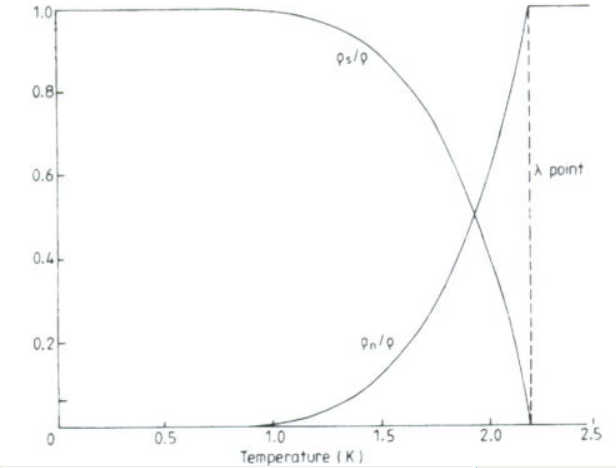
\includegraphics{./figures/twofluid.eps}
\caption{\small{Relative fractions $\rho_s/\rho$ and $\rho_n/\rho$ of
   the superfluid and normal components in He II.}}
\label{figure:twofluid}

\end{figure}
\end{center}


\subsection{Heat Transfer and Second Sound}

\subsubsection{Thermal Conductivity}
The thermal conductivity of He II is very high, and tends to infinity
for small heat currents \cite{tilley}, making the fluid intolerant
to temperature gradients. This property explains the visually
noticeable transition from He I to He II with decreasing temperature:
while in He I, there is a lot of bubbling, as the temperature drops
past the $\lambda$-point, the bubbling ceases immediately, since a
temperature gradient large enough cannot be established in order for a
bubble to form \cite{tilley}.


\subsubsection{Frictionless Flow}
Another property of helium II is that the superfluid component is able
to flow without energy dissipation. Since superfluid flows with zero
friction, it is possible to construct a barrier which permits
superfluid, but not normal fluid, to flow - such as tightly pressed
crushed glass which creates winding paths on the order of $100$
$\mu$m. Then, if a temperature gradient is established across such a
barrier, the only possible flow is superfluid flow, and the superfluid
will flow toward the higher temperatures in order to reduce the
gradient. As a qualitative demonstation of this property, our
experiment seeks to observe the `fountain' effect, where the
superfluid rushes through the barrier with enough pressure to create a
fountain on the opposite side.

\subsubsection{Second Sound}
Interestingly, the superfluid fraction cannot directly transfer heat,
but is able to balance temperature gradients not through the standard
methods of conduction and convection but through an exchange of the
relative concentrations of the two componenets $\rho_n$ and
$\rho_s$. As seen in FIGURE TWOFLUID, at lower temperatures the
fraction of superfluid increases and the fraction of normal fluid
decreases, so it is possible to think of the superfluid component as
`cold' and the normal component as `hot' \cite{atkins}. Thus, instead
of balancing temperature, it is possible to equivalently balance the
relative fraction of superfluid and normal fluid in different
reagions: superfluid flows up temperature gradients while normal fluid
flows toward lower temperatures to accomplish this.

This method of heat propagation in He II leads directly to the
definition of a different kind of wave possible in the fluid: second
sound. The term is defined in contrast to sound, known as first sound,
which is a pressure wave and travels via a variation of
density. Second sound is a temperature wave, and propagates instead
via a out of phase movement of superfluid and normal fluid past each
other, with constant total density at each point.

The relationship between velocity of second sound, $u_2$, and the
relative fractions of the fluids was derived analytically by Landau
and is given by

\begin{equation}
u_2^2 = \frac{\rho_s}{\rho_n}\frac{T S^2}{C}
\end{equation}

where $S$ and $C$ are the entropy and heat capacity per gram of the
liquid and can be measured experimentally \cite{atkins}. The
speed of second sound decreases with increasing temperature, going
to zero at the $\lambda$-point, where the superfluid fraction
dissapears.

\subsection{Heat Capacity}

\subsubsection{Specific Heat of Metals}

Accoring to the BLANK THEORY CITE HERE, two factors contribute to the
specific heat of metals. One, which is BLAH BLAH, increases linearly with temperature:
\begin{equation}
C_v() = \alpha T
\end{equation}

and the other is a cubed relationship
\begin{equation}
C_v() = \beta T^3
\end{equation}

giving a total specific heat of
\begin{equation}\label{formula:cuspecificheat}
C_v() =  \alpha T + \beta T^3
\end{equation}

where $\alpha$ and $\beta$ are constants that depend on the material
and are determined experimentally. This model is especially accurate
at low temperatures, and we use the relationship in
\ref{formula:cuspecificheat} to fit the heat capacity of the copper
cell which holds the liquid helium.

\subsubsection{Specific Heat of Liquid Helium}

The temperature dependence of the heat capacity of liquid helium is
unique to the system. The transition point from helium I to helium II
is named after the heat capacity dependece: the plot of heat capacity
versus temperature resembles the letter $\lambda$. Below $1$ K, the
heat capacity is nearly $0$; as the temperature increases from $1$ to
$2.17$K, the heat capacity increases rapidly, with an apparent
discontinuity at the $\lambda$-point, where heat capacity apparently
increases to infinity. Increasing the temperature still further, the
heat capacity drops to a minimum after the $\lambda$-point, and slowly
increases as the temperature reaches the helium boiling point p
31\cite{atkins}.

In our experiment, the specific heat was measured under the saturated
vapor pressure $C_{sat}$, which is related to the specific heat at constant pressure, $C_p$, by
\begin{equation}\label{formula:cuspecificheat}
C_{sat} = C_p - TV\alpha\left(\dfrac{dp}{dT}\right)_{v.p.c.} 
\end{equation}

where $\alpha$ is the coefficient of expansion and
$\left(\dfrac{dp}{dT}\right)_{v.p.c.}$ is the slope of the vapor
pressure curve \cite{atkins} p. 32. Accoring to Atkins, p. 32, below
$2.5$ K, the difference between $C_{sat}$ and $C_p$ is less than
$1\%$, but it increases to a significant fraction of $10\%$ at $4$
K. While it is difficult to control the volume and pressure of the
helium sample in our experiment, the liquid helium remains in
equilibrium with the helium vapor as temperature increases, and so we
are able to measure $C_{sat}$.

